\documentclass[11pt]{article}
\usepackage[margin=1in]{geometry}
\usepackage[T1]{fontenc}
\usepackage[utf8]{inputenc}
\usepackage{lmodern}
\usepackage{microtype}
\usepackage{graphicx}
\usepackage{booktabs}
\usepackage{amsmath}
\usepackage{xcolor}
\usepackage[numbers,sort&compress]{natbib}
\usepackage[hidelinks]{hyperref}
\usepackage{enumitem}
\setlist{itemsep=2pt,topsep=4pt}

% Every figure quoted in the text is generated from the run data by paper/make_numbers.py.
% Generated by paper/make_numbers.py. Do not edit by hand.
\newcommand{\NTables}{60}
\newcommand{\NNotes}{48}
\newcommand{\NMentions}{1,730}
\newcommand{\NChecked}{1,625}
\newcommand{\NSkipped}{105}
\newcommand{\NSkipEntity}{76}
\newcommand{\NSkipCount}{21}
\newcommand{\NSkipDate}{8}
\newcommand{\NCell}{1,367}
\newcommand{\NDerived}{255}
\newcommand{\NClaims}{1,613}
\newcommand{\NVerifiable}{1,613}
\newcommand{\NUnverifiable}{0}
\newcommand{\NGroupClaims}{69}
\newcommand{\SoneUnsupN}{3}
\newcommand{\SoneChecked}{514}
\newcommand{\SoneUnsup}{0.6\%}
\newcommand{\SoneBind}{0.0\%}
\newcommand{\VtwoSoneClaim}{0.6\%}
\newcommand{\SthreeRevised}{1}
\newcommand{\NotesErrSone}{1 of 12}
\newcommand{\FormatFail}{4}
\newcommand{\CostTotal}{\$2.54}
\newcommand{\CostPerNote}{\$0.053}
\newcommand{\NRawRows}{1,044,848}
\newcommand{\NCleanRows}{1,014,193}
\newcommand{\VoneSoneClaim}{9.3\%}
\newcommand{\VoneStwoClaim}{4.7\%}
\newcommand{\VoneSthreeClaim}{9.3\%}
\newcommand{\VoneSoneUnsup}{2.1\%}
\newcommand{\VoneFlags}{106}
\newcommand{\VoneLoneFlags}{22}
\newcommand{\VtwoLoneFlags}{3}
\newcommand{\VoneRatio}{16}
\newcommand{\CauseGroup}{47}
\newcommand{\CauseLevel}{26}
\newcommand{\CauseDirection}{20}
\newcommand{\CauseRest}{13}
\newcommand{\SuiteLoneItems}{379}
\newcommand{\SuiteLoneCorrect}{291}
\newcommand{\SuiteLoneFA}{2}
\newcommand{\SuiteLoneWrong}{88}
\newcommand{\SuiteLoneCaught}{61}
\newcommand{\SuiteLtwoItems}{203}
\newcommand{\SuiteLtwoFA}{0}
\newcommand{\SuiteLtwoWrong}{49}
\newcommand{\SuiteLtwoCaught}{49}
\newcommand{\HeldLone}{Fresh notes written independently of the gate rules, on tables the suites never used: 21 notes on 5 tables (526 numeric mentions) for Level~1, and 8 notes with 294 extractor-style claims on 8 tables for Level~2. At Level~1 the gate raised 22 false alarms on 353 correct numbers (6.2\%): 14 from gaps in the operation library (for example average order value for the whole table, or the rest of the table after the top $k$), 5 from rule gaps (for example ``gave up'' read as a rise) and 3 from entity names written with different spacing. It caught 79 of 111 wrong numbers (71\%). Of the 32 misses, 21 are real cells attached to the wrong row or period, which Level~1 cannot see by design, and 11 are rule gaps: 6 direction verbs missing from the lists (``plummeted'', ``rebounded''), 4 hedged bounds and 1 number written as ``c.137\%''. Excluding the by-design misses, it caught 88\%.}
\newcommand{\HeldLtwo}{At Level~2 it raised 8 false alarms on 202 correct claims (4.0\%), 4 of them from a single paraphrased product name matched to the wrong row, and detected 75 of 77 wrong claims (97\%), with the error type right for 71 of 75. Of 10 group figures, 6 were verified and 4 were falsely flagged because their subsets are not in the library.}
\newcommand{\HeldTwo}{Fresh notes written by agents that did not see the gate's rules, following the note-format prompt, on 15 tables no earlier test used, frozen by checksum before gate v3 (also checksummed) scored them; files in \texttt{paper/heldout2/}. Level~1 (28 notes, 681 numeric mentions): 7 false alarms on 435 correct numbers (1.6\%, Wilson 95\% interval 0.8\% to 3.3\%), from a level after ``down from'' read as a change (3), plural or one-word family names (3) and the mean of the rest of the table, which the library lacks (2). It caught 90 of 146 wrong numbers: 87 of 98 value errors (89\%; all 13 direction errors) but 3 of 48 binding errors, which Level~1 cannot see by design. Level~2 (18 notes, 417 claims written as a careful extractor would, so extractor errors are excluded): 6 false alarms on 270 correct claims (2.2\%, all per-order averages read as revenue), 3 correct claims lost as Unverifiable (a missing alias, UAE), and 99 of 104 wrong claims detected (95\%) with the error type right in all 99; 21 of 24 correct group figures and all 9 wrong ones were labelled correctly. Independent auditors re-derived a stratified random sample of 70 items per level from the tables and agreed with the recorded answer in all 140. Set~2 differs from set~1 in style (its notes follow the note-format rules, as real model output does) as well as in gate version, so the drop in false alarms from set~1 to set~2 is not a clean estimate of what v3's fixes achieved.}
\newcommand{\HeldTwoLoneFAPct}{1.6\%}
\newcommand{\HeldTwoLtwoFAPct}{2.2\%}
\newcommand{\PilotBaseRate}{0.18\%}
\newcommand{\HeldTwoRecall}{89\%}
\newcommand{\ExpectedPrecision}{9\%}
\newcommand{\FalsePerReal}{10}
\newcommand{\Adjudication}{We checked by hand, against the tables, every item the gate flagged in the pilot (3 unsupported numbers and 13 wrong claims under the gate at that point) and seeded random samples of 60 supported numbers and 60 correct claims. The 3 unsupported numbers were real errors, all in one sentence: a total for six parasol and umbrella lines reported as \pounds14,211.15 TW versus \pounds14,461.70 LW, a 1.7\% decline, where the six rows sum to \pounds17,211.15 and \pounds16,325.70, a 5.4\% rise. All 13 wrong claims were false alarms with three causes: group totals the extractor labelled TOTAL (6), a value found inside a longer number, such as 33 inside \pounds680.33 (4), and absolute changes read as levels, such as ``a decline of \pounds51.1k versus LW'' (3). The final gate fixes all three; on the pilot it flags exactly the 3 real errors at Level~1 and the same 3 as wrong group figures at Level~2, and nothing else. Because these fixes were made after seeing the pilot's flags, this agreement is not independent evidence of accuracy. The samples found no missed errors (0 of 60 numbers and 0 of 60 claims; a 95 percent upper bound of about 4.9 percent on the miss rate). One policy choice matters at this scale: six group shares equal the sum of the table's rounded Share\_Pct cells but miss the exact share at the cited precision (for example 37.2\% against an exact 37.13\%); we accept them as derivable from the table as shown, and counting them as errors would raise the pilot's unsupported count from 3 to 9 numbers (from 0.18 to 0.55 percent of checked numbers).}
\newcommand{\VoneFalsePct}{At least 97 percent}


\title{When the Checker Is Noisier Than the Model:\\Measuring Number Faithfulness in LLM-Written Business Notes}
\author{Author Name\\\small Affiliation\\\small \texttt{email@example.com}}
\date{Preprint, \today}

\begin{document}
\maketitle

\begin{abstract}
Executives increasingly read weekly performance notes drafted by large language models (LLMs) from sales tables, where one wrong number can mislead a decision. We present NumGate, an open, reproducible harness that measures how many numbers in such a note the source table does not support (number level) and how many claims attach a real number to the wrong entity, metric or period (claim level), using a two-level rule-based gate whose verdicts carry the supporting cell or operation. NumGate builds \NTables{} weekly report tables from the public UCI Online Retail II data and compares four generation strategies: direct writing, compute-then-write with code execution, write-then-verify, and a deterministic facts template. Our main result is about measurement. On the same \NNotes{} Claude Opus 5 notes, the first version of the gate reported a claim error rate of \VoneSoneClaim{} for direct writing, about \VoneRatio{} times the rate after correction, and \VoneFalsePct{} of its \VoneFlags{} claim flags were false alarms caused by ordinary phrasing. After two rounds of correction, the gate still raises false alarms on \HeldTwoLoneFAPct{} of correct numbers and \HeldTwoLtwoFAPct{} of correct claims in fresh held-out notes, which is far above the model's true error rate in our pilot (\SoneUnsupN{} wrong numbers in \NChecked{}; \NotesErrSone{} direct-writing notes contained a wrong sentence, and no note under the other strategies did). At that base rate only about \ExpectedPrecision{} of the gate's flags would be real errors. At the error rates of current models, the checker's accuracy dominates the measurement, so automatic faithfulness scores should be reported with the checker's measured precision. The pilot is too small to rank strategies or table sizes; we release the harness, prompts, gate rules, held-out test sets and data for the full study.
\end{abstract}

\section{Introduction}

Weekly business reviews summarise tables: revenue by country this week (TW) versus last week (LW) and the same week last year (LY), week over week (WoW) and year over year (YoY) changes, shares and ranks. LLMs are now used to draft these notes. The failure that matters most in this setting is not fluency or tone but a wrong number: a revenue figure attributed to the wrong country, a decline reported as growth, or a total that no row of the table supports.

Measuring this failure is harder than it looks. A note can cite a number that is not a cell but is correctly derived (a share, a total, a percent change), cite a correct number with the wrong label (last year's figure presented as last week's), or state the right number for the wrong entity. Scoring notes by hand does not scale across models, strategies and table sizes, and an automatic checker has its own error rate.

We ask four questions:
\begin{enumerate}[label=\textbf{RQ\arabic*}]
  \item What fraction of the numbers an LLM cites in an insight note are not supported by the table?
  \item What fraction of its claims bind a number to the wrong entity, metric or period?
  \item Which generation strategy reduces these rates most: direct writing, compute-then-write with code execution, or write-then-verify?
  \item How do the rates change with table size and model?
\end{enumerate}

This paper describes the measurement instrument and a pilot study with one model on six tables. The pilot addresses RQ1 and RQ2 for that model; it is too small to answer RQ3 and RQ4, which need the full study (three models, all \NTables{} tables, about \$60 at the pilot's measured cost per note). Our contributions are:
\begin{itemize}
  \item \textbf{NumGate}, a reproducible harness: a table builder over public retail data, four generation strategies behind one model interface with on-disk caching and a budget stop, a two-level number gate, analysis with bootstrap confidence intervals, and an interactive results dashboard.
  \item \textbf{A precise, rule-based number gate} whose rules fit in two pages (Section~\ref{sec:gate}) and whose verdicts carry evidence (the table cell or the operation that supports each number).
  \item \textbf{Pilot results} for Claude Opus 5 across the four strategies, at the number, claim and note level, confirmed by hand.
  \item \textbf{A measurement lesson}: on the same notes, a first version of the gate overstated claim errors by about \VoneRatio{} times. We categorise every false alarm, show the fixes, and measure each gate version on fresh held-out notes it was not revised on. We recommend that papers reporting LLM faithfulness rates also report the precision of their checker.
\end{itemize}

\section{Related work}

\paragraph{Faithfulness in data-to-text generation.} Table-to-text generation has long been evaluated for faithfulness to the source. \citet{wiseman2017challenges} introduced extractive evaluation of generated game summaries, including a relation-generation measure that extracts (entity, value, type) records from text and checks them against the source table, which is the closest precedent to our Level~2. ToTTo \citep{parikh2020totto} and PARENT \citep{dhingra2019parent} address faithful table-to-text generation and its evaluation. TabFact \citep{chen2020tabfact} frames the verification of statements against tables as a classification task. Our setting differs in three ways: the text is an executive note with many derived quantities, the checker is fully deterministic apart from claim extraction, and we evaluate generation strategies rather than models alone.

\paragraph{Hallucination detection.} Surveys document how often generated text states unsupported facts \citep{ji2023survey}. FActScore \citep{min2023factscore} decomposes long-form text into atomic facts and checks each, and SelfCheckGPT \citep{manakul2023selfcheckgpt} detects hallucination from sampling consistency. NumGate follows the decompose-and-check pattern, but its source of truth is a small table, so support can be decided exactly with a rounding rule.

\paragraph{Computing before writing, and verifying after.} Program-aided language models \citep{gao2023pal} and Program of Thoughts \citep{chen2023pot} have the model write code whose execution produces the numbers, which motivates our compute-then-write strategy. Self-Refine \citep{madaan2023selfrefine} and Chain-of-Verification \citep{dhuliawala2024cove} have the model critique or verify its own draft; our write-then-verify strategy instead feeds back the flags of an external deterministic checker.

\section{Task and data}
\label{sec:data}

\paragraph{Source.} We use UCI Online Retail II \citep{chen2019onlineretail}: invoice lines of a UK online gift retailer from December 2009 to December 2011, with invoice, stock code, description, quantity, date, unit price, customer and country. The data come as two yearly sheets that overlap in early December 2010; keeping each invoice once leaves \NRawRows{} lines. We drop cancelled invoices, rows with non-positive quantity or price, rows without a country and non-product stock codes (postage, bank charges and similar), leaving \NCleanRows{} rows. Revenue is quantity times unit price, in GBP.

\paragraph{Report tables.} We aggregate to ISO weeks. Each table lists the top $N$ entities of one week by revenue, with columns Entity, Revenue\_TW, Revenue\_LW, Revenue\_LY, Units\_TW, Units\_LW, Orders\_TW, Orders\_LW, WoW\_Pct, YoY\_Pct, Share\_Pct and Rank. All derived columns are computed from the rounded stored columns, so every derived cell recomputes exactly from the CSV. Tables come in three sizes: small (5 to 10 rows), medium (20 to 40) and large (80 to 150). Countries fill only small tables (a typical week has about 13 trading countries), so medium and large tables list products. With a fixed seed we build \NTables{} tables: 20 small (10 country, 10 product), 20 medium and 20 large.

\section{Generation strategies}
\label{sec:strategies}

All strategies produce the same note format, enforced by the prompt: 6 to 8 bullet lines, one insight per line, each naming an entity and containing at least one number, with periods labelled explicitly (TW, LW, LY, WoW, YoY), facts only and no recommendations. All prompts are released with the harness.

\begin{description}
  \item[S1 Direct.] The table is given as a markdown table; the model writes the note in one call.
  \item[S2 Compute-then-write.] The model writes a short pandas script that computes up to 25 facts (entity, metric, period, value, formula). The script runs in a subprocess with a 30 second timeout; on failure it is retried once with the error message. A second call writes the note from the facts alone, without the table.
  \item[S3 Write-then-verify.] The S1 draft is scored by the Level~1 gate; unsupported numbers are sent back with the table for correction or removal, for at most two rounds.
  \item[S4 Facts-template.] A deterministic pandas facts packet (totals, top three entities, largest WoW and YoY movers, most orders) is narrated with every number copied verbatim. S4 is an upper bound on what a gated design can reach, not a free-generation strategy.
\end{description}

\section{The number gate}
\label{sec:gate}

The gate is deterministic except for claim extraction. Full rules with worked examples are in the released method document; we summarise them here.

\paragraph{Level 1: number support.} A single regular expression extracts every numeric mention with its value, cited precision, unit (currency, percent, count, plain), sign and hedge. Signs come from explicit signs (including an en dash used as a minus) or from direction words (fell, rose, down) before or after the number, but a level word (to, from, at) between a direction word and the number makes it a level: in ``fell to \pounds1,632.90 TW'' the amount is unsigned. Numbers that are not measurements are skipped with a recorded reason: digits inside entity names, week labels, years and counting phrases (``top 3'', ``2 of the 5 countries''). A cited value $c$ matches a true value $t$ when $t$ rounds half-up to it at the cited precision, $-h \le |t|/s - |c| < h$ with $h = 0.5 \cdot 10^{-d}$ for scale $s$ and $d$ decimals, and signed values agree in sign; values written with k, M or B also match within 0.5 percent, hedged values (``about'') within 5 percent. Each number is compared, in order, with (1) cells of the entities named in its line, (2) values derived from those entities and from the groups and product families the line mentions (changes, shares, share-point changes, per-order values, totals of the rest of the table, family sums), (3) table-level aggregates when the line names no entity or uses an aggregate word, and (4) any other cell. The first match labels the number Supported\_cell or Supported\_derived with its evidence; otherwise it is Unsupported. Anchoring derived values on the entities named in the line keeps the candidate set small: in a 150-row table, unrestricted pairwise operations would match almost any number by chance.

\paragraph{Level 2: claim binding.} A cheap model (Claude Haiku 4.5 in our pilot) extracts one claim per number, (entity, metric, period, value, direction, qualifier), with a fixed JSON schema and prompt. The extractor only transcribes; values are re-parsed by the Level~1 parser. Labels written in the note override the extractor: a period label adjacent to a value (``\pounds2,729.22 LW'') sets its period, change wording (``a decline of \pounds51.1k'') marks it as a change, and a unit noun (``8 orders'') sets its metric; values are located only where they stand alone, so 33 is not found inside \pounds680.33. Each claim is resolved to one or more rows (exact name, aliases and demonyms, word-subset match, fuzzy match with ties kept) and to a column, and labelled Correct; Wrong\_value if only the sign differs or nothing matches; Wrong\_metric if the value belongs to another column of the same row (for example the YoY figure cited as WoW); Wrong\_entity if it belongs to the same column of another row that the line names, or of exactly one other row; and Unverifiable for names that fit several rows none of which matches and for metrics the table cannot answer. Group figures (``the three parasol lines combined'', ``the top five''), including subsets the extractor mislabels as the whole-table total, are checked against the same group, product-family, top-k and table totals that Level~1 uses for the line, and are labelled Correct or Wrong\_value.

\paragraph{Metrics.} The \emph{unsupported rate} is Unsupported over checked numbers (RQ1). The \emph{binding error rate} is (Wrong\_entity + Wrong\_metric) over verifiable claims (RQ2). The \emph{claim error rate} adds Wrong\_value. Rates are pooled over the notes of a group, with 95 percent percentile bootstrap intervals from 1,000 resamples of notes \citep{efron1993bootstrap}; strategy differences use a paired bootstrap over conditions matched on table, model and repeat.

\section{Pilot study}
\label{sec:pilot}

\paragraph{Setup.} The pilot runs Claude Opus 5 on the smoke set: two tables of each size (\NTables{}-table pool, seeded selection), four strategies and two repeats, \NNotes{} notes in all. Opus 5 does not accept a temperature parameter and thinks adaptively by default, so repeats sample independently. Every response is cached, and the repeat index is part of the cache key. The pilot's note generation cost \CostTotal{} (\CostPerNote{} per note on average).

\paragraph{Scale of the pilot.} The \NNotes{} notes contain \NMentions{} numeric mentions: \NChecked{} were checked and \NSkipped{} skipped (\NSkipEntity{} inside entity names, \NSkipCount{} counting phrases, \NSkipDate{} week labels). Of the checked numbers, \NCell{} matched a cell and \NDerived{} a derived value. The extractor returned \NClaims{} claims, of which \NVerifiable{} were verifiable, including \NGroupClaims{} group figures checked against group totals.

\begin{table}[t]
\centering
\caption{Pilot results for Claude Opus 5 (\NNotes{} notes; gate v3). Rates pool numbers or claims over notes; brackets give 95 percent bootstrap intervals over notes. With 12 notes per strategy the intervals are wide.}
\label{tab:pilot}
\resizebox{\linewidth}{!}{%
\begin{tabular}{lrrrrrrr}
\toprule
Strategy & Numbers & Unsupported \% & Claims & Wrong entity or metric \% & Any claim error \% & Notes with an error & Cost per note \\
\midrule
S1 Direct & 514 & 0.6 [0.0, 2.0] & 508 & 0.0 [0.0, 0.0] & 0.6 [0.0, 2.2] & 1 / 12 & \$0.049 \\
S2 Compute-then-write & 301 & 0.0 [0.0, 0.0] & 301 & 0.0 [0.0, 0.0] & 0.0 [0.0, 0.0] & 0 / 12 & \$0.095 \\
S3 Write-then-verify & 514 & 0.0 [0.0, 0.0] & 508 & 0.0 [0.0, 0.0] & 0.0 [0.0, 0.0] & 0 / 12 & \$0.053 \\
S4 Facts-template & 296 & 0.0 [0.0, 0.0] & 296 & 0.0 [0.0, 0.0] & 0.0 [0.0, 0.0] & 0 / 12 & \$0.015 \\
\bottomrule
\end{tabular}}

\end{table}

\paragraph{Results.} Table~\ref{tab:pilot} gives the pilot rates. Opus 5 cited very few unsupported numbers: \SoneUnsupN{} of \SoneChecked{} under direct writing (\SoneUnsup{}), all in one sentence that reported a wrong total for a product family, and none under the other strategies. At the note level, which is what a reader of the note experiences, \NotesErrSone{} direct-writing notes contained a wrong sentence and no note under the other strategies did. No claim under any strategy attached a number to the wrong entity, metric or period; the only claim errors are the same three group figures. Section~\ref{sec:validation} confirms these verdicts by hand. Write-then-verify revised \SthreeRevised{} of 12 drafts: the draft that contained the pilot's only real error, a total for six parasol and umbrella lines. The revision did not correct that total; it replaced the claim with a narrower one, a total for the three EDWARDIAN PARASOL colourways only (\pounds9,139.25 TW versus \pounds9,454.25 LW, a 3.3\% decline), which is correct. Removing or narrowing a flagged claim, rather than fixing it, is a behaviour a verify loop can reward. The facts template produced the shortest and cheapest notes. Table~\ref{tab:size} breaks the pilot down by table size: all errors fall in one medium table, and with two tables per size no size effect can be read from it. \FormatFail{} of \NNotes{} notes broke the 6 to 8 bullet rule, all on one small country table with six rows, where the model wrote fewer bullets than asked. These rates are far lower than the ones our first gate reported, which is the subject of the next section.

\begin{table}[t]
\centering
\caption{Pilot results by table size (all four strategies pooled; two tables per size).}
\label{tab:size}
\begin{tabular}{lrrrrrrr}
\toprule
Table size & Tables & Notes & Numbers & Unsupported (\%) & Claims & Claim errors & Notes with an error \\
\midrule
small & 2 & 16 & 440 & 0 (0.0) & 438 & 0 & 0 / 16 \\
medium & 2 & 16 & 576 & 3 (0.5) & 572 & 3 & 1 / 16 \\
large & 2 & 16 & 609 & 0 (0.0) & 603 & 0 & 0 / 16 \\
\bottomrule
\end{tabular}

\end{table}

\begin{figure}[t]
\centering
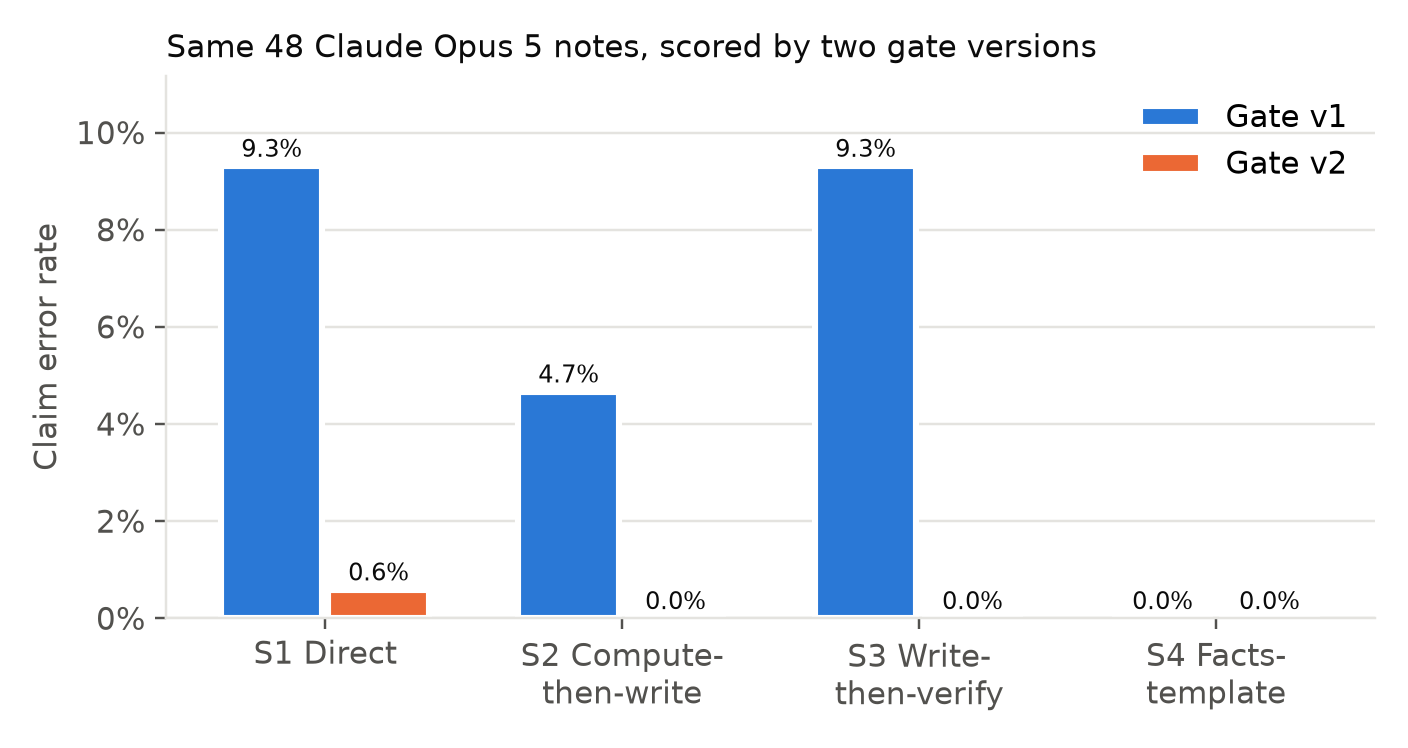
\includegraphics[width=0.49\linewidth]{figures/fig_v1_v2.png}\hfill
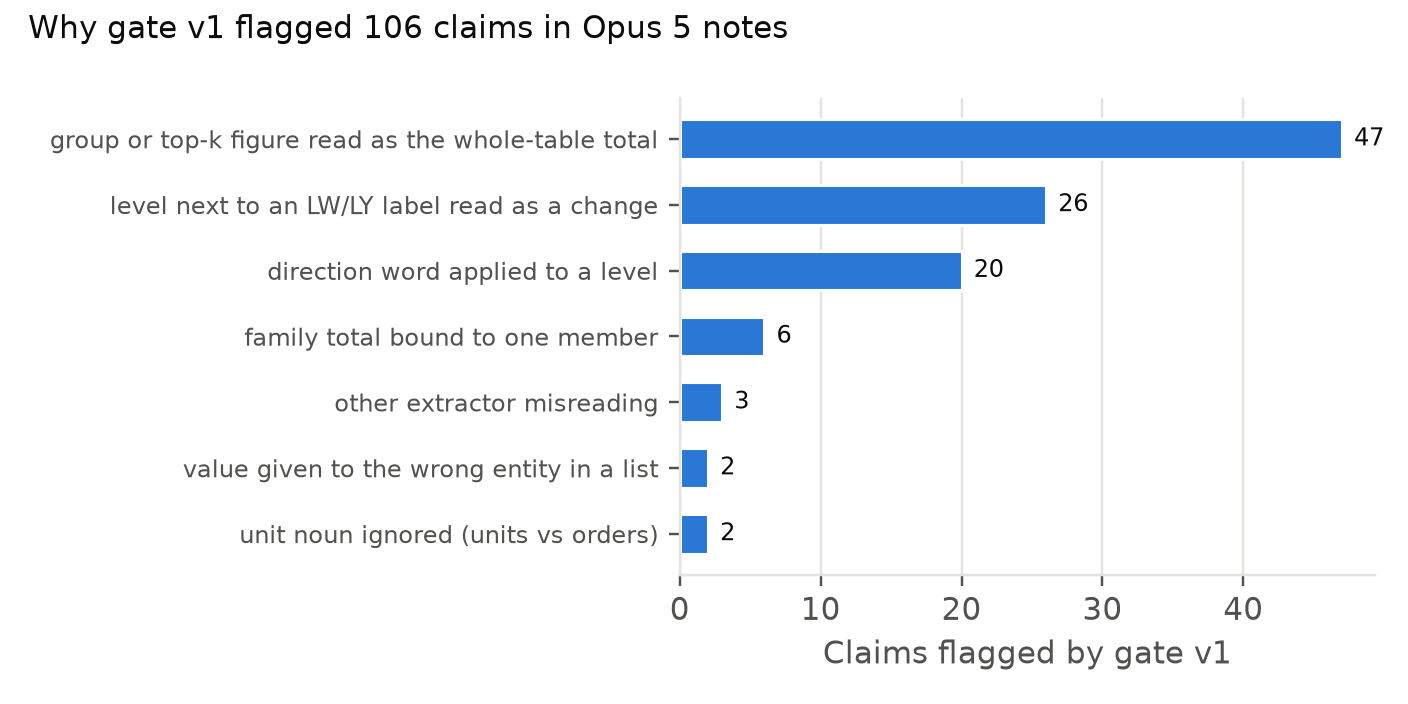
\includegraphics[width=0.49\linewidth]{figures/fig_v1_causes.png}
\caption{Left: claim error rate on the same \NNotes{} Opus 5 notes under gate v1 and gate v2. Right: why gate v1 flagged its \VoneFlags{} claims. Almost all v1 flags were false alarms caused by ordinary phrasing.}
\label{fig:v1v2}
\end{figure}

\section{How much of the measured error is the checker's?}
\label{sec:v1}

The first version of the gate (v1) was developed on a mock model that writes template notes with planted errors, where it caught every planted error. On the real Opus 5 notes it reported claim error rates of \VoneSoneClaim{} (S1), \VoneStwoClaim{} (S2) and \VoneSthreeClaim{} (S3), and an S1 unsupported rate of \VoneSoneUnsup{}. Reading the flagged sentences showed that nearly all were correct. Figure~\ref{fig:v1v2} categorises the \VoneFlags{} flagged claims:
\begin{itemize}
  \item \textbf{Group or top-k figures read as the whole-table total} (\CauseGroup{}). ``The top five TW products combined for 16.9\% share'' was extracted with entity TOTAL and compared with the total's 100 percent share.
  \item \textbf{A level next to an LW or LY label read as a change} (\CauseLevel{}). In ``\pounds3,205.71 TW versus \pounds2,729.22 LW (WoW +17.5\%)'' the extractor gave the LW amount the period WoW.
  \item \textbf{A direction word applied to a level} (\CauseDirection{}). In ``fell to \pounds1,632.90 TW'' the level was signed negative and failed to match.
  \item \textbf{Family totals bound to one member, unit nouns ignored, list order} (\CauseRest{} together): ``the three EDWARDIAN PARASOL colourways combined'' matched the BLACK product; ``140 units and 8 orders'' gave 8 the metric units; a ``respectively'' list was assigned out of order.
\end{itemize}
The fixes are small and general: directions sign only changes; a label written next to a value overrides the extractor; the extractor marks group figures as GROUP and Level~1 knows family and group totals; ambiguous short names are checked against every row they fit; and a same-row mix-up is tested before a different-row one. Gate v2 reports \VtwoSoneClaim{} for S1 on the same notes, and its Level~1 flags fell from \VoneLoneFlags{} to \VtwoLoneFlags{}.

The lesson generalises beyond this harness. When a model's true error rate is around one percent, a checker with a false alarm rate of a few percent per claim produces a measured error rate several times the true one, and differences between strategies can be artefacts of which phrasings each strategy tends to use. A checker validated only on synthetic errors (our mock) can look perfect and still fail on real text.

\section{Validating the gate}
\label{sec:validation}

The gate went through three versions. Gate v1 was built on the mock model. Gate v2 was revised after reading v1's flags on the pilot, and was then measured on a first set of fresh held-out notes. Gate v3 was revised using that held-out set's diagnoses and the pilot adjudication, frozen (its source file's checksum is recorded), and measured on a second held-out set written on tables no earlier test used. Each held-out set therefore measures a gate that was not revised on it; every other row of Table~\ref{tab:validation} measures a gate on text its rules were revised on. A human audit, described last, is the definitive test.

\begin{table}[t]
\centering
\caption{Accuracy of the gate on its test sets. False alarms are correct numbers (L1) or claims (L2) flagged as errors; caught errors are deliberately wrong (or, for the pilot, adjudicated wrong) numbers and claims that were flagged. Only the held-out rows measure a gate on text its rules were not revised on.}
\label{tab:validation}
\begin{tabular}{lrrrr}
\toprule
Test set & L1 false alarms (\%) & L1 errors caught (\%) & L2 false alarms (\%) & L2 errors detected (\%) \\
\midrule
Regression suites, gate v3 (rules tuned on them) & 2 / 291 (0.7) & 61 / 88 (69) & 0 / 149 (0.0) & 49 / 49 (100) \\
Held-out set 1, gate v2 & 22 / 353 (6.2) & 79 / 111 (71) & 8 / 202 (4.0) & 75 / 77 (97) \\
Held-out set 2, gate v3 & 7 / 435 (1.6) & 90 / 146 (62) & 6 / 270 (2.2) & 99 / 104 (95) \\
Opus pilot, gate v3, adjudicated (rules revised on it) & 0 / 1,622 (0.0) & 3 / 3 (100) & 0 / 1,610 (0.0) & 3 / 3 (100) \\
\bottomrule
\end{tabular}

\end{table}

\paragraph{Regression stress suites.} Two suites written in varied LLM styles, with ground truth computed from the tables, test Level~1 on \SuiteLoneItems{} numbers and Level~2 on \SuiteLtwoItems{} claims. Gate v3 raises \SuiteLoneFA{} false alarms on \SuiteLoneCorrect{} correct numbers and catches \SuiteLoneCaught{} of \SuiteLoneWrong{} wrong ones; most of the misses are real cells attached to the wrong row or period, which Level~1 cannot see by design and Level~2 catches. At Level~2 it raises \SuiteLtwoFA{} false alarms and detects \SuiteLtwoCaught{} of \SuiteLtwoWrong{} wrong claims. Because the fixes were developed while looking at these suites, we report them as regression tests, not as accuracy estimates.

\paragraph{Held-out set 1 (gate v2).} \HeldLone{} \HeldLtwo{} The scripts for this set were written in a temporary folder that was later deleted, so only its recorded results survive; set 2 is saved in the repository.

\paragraph{Held-out set 2 (gate v3).} \HeldTwo{}

\paragraph{Adjudication of the pilot.} \Adjudication{}

\paragraph{Human audit.} The harness samples 200 numbers and 200 claims, stratified by strategy and label, for a human audit and reports per-label precision and recall. This audit is the definitive test of the gate for the full study and is not yet complete.

\section{Discussion and limitations}

\paragraph{What the pilot says.} On small weekly tables, a frontier model writes executive notes whose numbers are almost always supported, and the strategies that compute or copy numbers remove the remaining unsupported ones. Whether this holds for other models, larger tables and the full table pool is what the full study measures (the harness estimates about \$57 for three models, 60 tables, four strategies and two repeats).

\paragraph{What the gate's own error rate implies.} The pilot's true error rate (\SoneUnsupN{} wrong numbers in \NChecked{}, \PilotBaseRate{}) is far below the gate's false alarm rate on fresh held-out text: 6.2 percent of correct numbers and 4.0 percent of correct claims for gate v2 on set 1, and \HeldTwoLoneFAPct{} and \HeldTwoLtwoFAPct{} for gate v3 on set 2. Bayes' rule makes the consequence concrete. With set~2's false alarm rate (\HeldTwoLoneFAPct{}) and value-error recall (\HeldTwoRecall{}), a Level~1 flag at the pilot's base rate would be a real error only about \ExpectedPrecision{} of the time, roughly \FalsePerReal{} false flags for every real one. The pilot's three flags were all real only because the gate's rules had been revised on those very notes. Two readings are consistent with our data: real model notes, constrained by the note format, may use fewer of the phrasings that trip the gate than our deliberately varied held-out notes do; or the pilot's zero false alarms reflect rules revised on the pilot itself. Either way, raw gate rates cannot be compared across models or strategies at this scale without an estimate of the gate's precision on the same notes. For the full study we therefore report gate rates together with human-audited precision per strategy, and treat the gate as a triage tool whose flags are confirmed by a person.

\paragraph{Limitations.}
\begin{itemize}
  \item \textbf{Pilot size.} 48 notes from one model on six tables; the intervals are wide and no strategy difference is significant. The final gate's rules were revised after seeing the pilot's flags, so its agreement with the adjudication on the pilot is not independent evidence; the held-out tests and the human audit are.
  \item \textbf{One data domain.} A single UK online retailer, weekly grain, GBP, and country and product entities.
  \item \textbf{Known gaps in gate v3.} Held-out set~2 found: per-order averages cited as money are read as revenue at Level~2; a level after ``down from'' is read as a change; plural or one-word family names (``cushions'', ``MUG'') are not recognised as families; the mean of the rest of the table is not in the library; bounds are not allowed on group figures; and some aliases (UAE) are missing. Fixing them requires a third held-out set to measure the result honestly.
  \item \textbf{Gate coverage.} Numbers written as words (``doubled'') are not extracted; derived values outside the operation library are Unsupported (the held-out tests found gaps such as table-level average order value and the rest of the table after the top $k$); some direction verbs (``plummeted'', ``rebounded'') are missing from the lists; hedged bounds (``more than'') can be satisfied by an unrelated column of the named row; paraphrased product names can bind to the wrong row; superlatives (``the largest swing'') are not checked; the 0.5 percent tolerance for k and M values accepts a wrong last digit at large scales; truncated values without k or M count as unsupported.
  \item \textbf{Extractor dependence.} Level~2 inherits the extractor's errors, and a value assigned to the wrong entity in a list can still produce a false Wrong\_entity.
  \item \textbf{S3 and its scorer.} Write-then-verify is revised against the Level~1 gate that also scores it, so its Level~1 rate is biased low; Level~2 and the human audit are the fairer comparison.
\end{itemize}

\section{Reproducibility}

The harness is plain Python with pandas. Tables are rebuilt from the UCI download with a fixed seed and every derived column is checked on build. Every model response is cached on disk, keyed by model, prompts, temperature and repeat, so rerunning any experiment is free; a budget cap stops a run and a rerun resumes it. \texttt{run\_all} builds the tables, runs a smoke experiment with a mock model (no API key), analyses it and opens the dashboard. The pilot is reproduced by \texttt{run\_experiment.py --models claude-opus-5 --tables-per-size 2 --run-id smoke\_opus}, the v1 comparison by \texttt{paper/rescore\_v1.py}, and every number in this paper by \texttt{paper/make\_numbers.py}.

\bibliographystyle{plainnat}
\bibliography{references}

\end{document}
